% Change to 'masters' to produces the masters thesis preliminary pages
\documentclass[oneside]{book}

\usepackage{import}

% preamble contains title page, signature page, acknowledgment and abstract texts
% Modify this file to complete your dissertation
\ProvidesPackage{preamble}

\usepackage{amsmath}
\usepackage{ifpdf}

\ifpdf
  \usepackage[pdftex]{graphicx}
\else
  \usepackage[dvips]{graphicx}
\fi

\usepackage{afterpage}
\usepackage{rotating}
%\usepackage{subfigure}
% Change the CLASS FILE from WSUclass to bookbinding (and edit class file names accordingly) after your thesis is turned in electronically so you can get your dissertation bound and don't forget to change the above from oneside to twoside!!!!!!!!!!!!!!
\usepackage{fancyhdr}
  \fancyfoot[C,CO]{\textbf{\thepage}}
  \pagestyle{plain}
  \renewcommand{\chaptermark}[1]{\markboth{\chaptername \ \thechapter \ \ #1}{}}
  \renewcommand{\sectionmark}[1]{\markright{\thesection \ \ #1}}

% The caption package allows us to change the formatting of figure captions.
% The commands here change to the suggested caption format: single spaced and a bold tag
\usepackage[margin=0.3in,labelfont=bf,labelsep=none]{caption}
 \DeclareCaptionFormat{suggested}{\singlespace#1#2 #3\par\doublespace}
 \captionsetup{format=suggested}

% The cite package cleans up the way citations are handled.  For example, it
% changes the citation [1,2,3,6,7,8,9,10,11] into [1-3,6-11].  If your advisor
% wants superscript citations, use the overcite package instead of the cite package.
%\usepackage{cite}

% The makeidx package makes your index for you.  To make an index entry,
% go to the place in the book that should be referenced and type
%  \index{key}
% An index entry labeled "key" (or whatever you type) will then
% be included and point to the correct page.
\usepackage{makeidx}


\makeindex

% The url package allows for the nice typesetting of URLs.  Since URLs are often
% long with no spaces, they mess up line wrapping.  The command \url{http://www.physics.byu.edu}
% allows LaTeX to break the url across lines at appropriate places: e.g. http://www.physics.byu.edu
\usepackage{url}
\urlstyle{rm}

% The hyperref package provides automatic linking and bookmarking for the table
% of contents, index, equation references, and figure references.
%
% To include a link in your pdf use \href{URL}{Text to be displayed}.  If your
% display text is the URL, you probably should use the \url{} command discussed
% above.
%
% To add a bookmark in the pdf you can use \pdfbookmark.  You can look up its usage
% in the hyperref package documentation
\usepackage[bookmarksnumbered,pdfpagelabels=true,plainpages=false,colorlinks=true,
            linkcolor=black,citecolor=black,urlcolor=blue]{hyperref}

%   \makepreliminarypages : Makes the preliminary pages
%   \clearemptydoublepage : same as \cleardoublepage but doesn't put page numbers
%                           on blank intervening pages
%   \singlespace          : switch to single spaced lines
%   \doublespace          : switch to double spaced lines
\newcommand{\bibs}{DissertationRefs}
\newcommand{\comments}[1]{}

% ==================================================== %
%                                                      %
%   Fill in these fields for the preliminary pages     %
%                                                      %
% ==================================================== %

% For Senior and honors this is the year and month that you submit the thesis
% For Masters and PhD, this is your graduation date
  \Year{2018}
  \Month{May}
  \Author{Jane Mary Loe}
  \University{Washington State University}
  \Department{School of Electrical Engineering and Computer Science}
  \DegreeShort{Ph.D.}

% If you have a long title, split it between two lines. The \TitleBottom field defines the second line
% A two line title should be an "inverted pyramid" with the top line longer than the bottom.
  \TitleTop{Your Title Goes Here}
  \TitleMiddle{}
  \TitleBottom{ }

% Your research advisor
  \Advisor{Rudyard Kipling}
  \AdvisorTitle{Ph.D.}

% The representative of the department who will approve your thesis (usually the chair) THIS DOESN'T MATTER FOR WSU
  \DepRep{}
  \DepRepTitle{}

% Acknowledge those who helped and supported you
  \Acknowledgments{
Nullam mollis et leo at pharetra. Nulla efficitur molestie euismod. Sed dapibus metus sed tempus varius. Aenean finibus eros ut urna luctus feugiat. Duis turpis risus, viverra vitae porta et, ullamcorper ac est. Proin in eros nec ipsum interdum tempus. Nam fringilla lectus velit, non posuere ex vehicula ut. Mauris tincidunt, dolor sit amet commodo tempor, erat mi egestas dui, at elementum tellus est rhoncus libero. Ut et rutrum lectus, id viverra tortor. Vivamus nec lacus eros. Donec dictum porta nisi et vestibulum. Mauris luctus ligula ut libero aliquet luctus. Quisque malesuada egestas finibus. 

Mauris dictum pharetra fermentum. Maecenas ut felis varius, dapibus sapien imperdiet, dictum dui. Proin feugiat viverra metus non laoreet. Integer pulvinar mi id lacus semper commodo. Praesent vel erat interdum purus scelerisque maximus. Sed enim risus, mollis blandit ligula ac, sagittis venenatis augue. Mauris nisi purus, gravida ac aliquam eu, ullamcorper eget nulla. Proin id finibus purus. Vestibulum leo ante, porta in quam sed, eleifend feugiat arcu. Nunc viverra fringilla turpis a iaculis. In condimentum aliquet mauris, quis laoreet eros porta eu. Aenean ut turpis a massa gravida pretium. Phasellus auctor purus quis diam interdum, nec luctus lorem auctor. Pellentesque finibus elit justo, a vulputate diam fermentum lacinia. 

}


% The text of your abstract
% Known bugs
%   Having a tiny bit of the abstract spill to second page defeats page number removal.
%   Workaround: make the abstract a little longer or a little shorter.
%
  \Abstract{
Nullam mollis et leo at pharetra. Nulla efficitur molestie euismod. Sed dapibus metus sed tempus varius. Aenean finibus eros ut urna luctus feugiat. Duis turpis risus, viverra vitae porta et, ullamcorper ac est. Proin in eros nec ipsum interdum tempus. Nam fringilla lectus velit, non posuere ex vehicula ut. Mauris tincidunt, dolor sit amet commodo tempor, erat mi egestas dui, at elementum tellus est rhoncus libero. Ut et rutrum lectus, id viverra tortor. Vivamus nec lacus eros. Donec dictum porta nisi et vestibulum. Mauris luctus ligula ut libero aliquet luctus. Quisque malesuada egestas finibus. 

Mauris dictum pharetra fermentum. Maecenas ut felis varius, dapibus sapien imperdiet, dictum dui. Proin feugiat viverra metus non laoreet. Integer pulvinar mi id lacus semper commodo. Praesent vel erat interdum purus scelerisque maximus. Sed enim risus, mollis blandit ligula ac, sagittis venenatis augue. Mauris nisi purus, gravida ac aliquam eu, ullamcorper eget nulla. Proin id finibus purus. Vestibulum leo ante, porta in quam sed, eleifend feugiat arcu.
}

% The text of your dedication
% This page is OPTIONAL. To remove, comment out \dedicationpage in diss.tex
  \Dedication{
    This dissertation/thesis is dedicated to my mother and father who \\ provided both emotional and financial support
}


% ------------- These remaining fields are only necessary for masters and PhD ----------------------

% The members of your graduate committee (masters only need A and B, PhD need all 4)
  \MemberA{Jane Austin}
  \MemberATitle{Ph.D.}
  \MemberB{John F.\ Kennedy}
  \MemberBTitle{Ph.D.}



% Revision: 02-01-2018
% Revision History
%   02-01-2018 : Follow WSU PhD/Masters format requirements as of 02-01-2018
%   07-10-2008 : Corrected Alignment of signature boxes on Masters/PhD Approval page
%   07-25-2007 : Corrected some spelling errors
%   05-16-2006 : Added etd option and moved most packages from class file to template
%   05-15-2006 : Initial version.
%
% Known bugs
%   Having a tiny bit of the abstract spill to second page defeats page number removal.
%   Workaround: make the abstract a little longer or a little shorter.
%
% You can supply
% the following optional arguments in the square brackets to
% specify the thesis type:
%
%   senior  : Produces the senior thesis preliminary pages (default)
%   honors  : Produces the honors thesis preliminary pages
%   masters : Produces the masters thesis preliminary pages
%   phd     : Produces the PhD dissertation preliminary pages
%
% The default format is appropriate for printing, with blank pages
% inserted after the preliminary pages in twoside mode so you can
% send it directly to a two-sided printer. However, for ETD
% submission the blank pages need to be removed from the final output.
% The following option does this:
%
%   etd     : Produces an electronic copy with no blank pages in the preliminary section
%
% The rest of the class options are the same as the regular book class.
% A few to remember:
%
%   oneside : Produces single sided print layout (recommended for theses less than 50 pages)
%   twoside : Produces single sided print layout (the default if you remove oneside)
%
% The BYUPhys class provides the following macros:
%
%   \makepreliminarypages : Makes the preliminary pages
%   \clearemptydoublepage : same as \cleardoublepage but doesn't put page numbers
%                           on blank intervening pages
%   \singlespace          : switch to single spaced lines
%   \doublespace          : switch to double spaced lines
%
% ------------------------------------------------------------------------------------------------------
%
\NeedsTeXFormat{LaTeX2e} \ProvidesClass{WSUclass}

% ---------------------------- declarations -------------------------
%
% These macros are used to declare arguments needed for the
% construction of the preliminary pages

% Fix?
\newcommand{\cedp}{\newpage{\pagestyle{empty}
\cleardoublepage}}

% The year and month the degree is awarded
\newcommand{\Year}[1]{\gdef\@Year{#1}}
\newcommand{\Month}[1]{\gdef\@Month{#1}}

% The full name of the degree
\newcommand{\degree}[1]{\gdef\@degree{#1}}

% The full name of the degree
\newcommand{\DegreeShort}[1]{\gdef\@DegreeShort{#1}}

% The name of this document (thesis/dissertation)
\newcommand{\docname}[1]{\gdef\@docname{#1}}

% First line of title
\newcommand{\TitleTop}[1]{\gdef\@TitleTop{\mbox{\uppercase{#1}}}}

%Middle line of title
\newcommand{\TitleMiddle}[1]{\gdef\@TitleMiddle{\mbox{\uppercase{#1}}}}

% Second line of title
\newcommand{\TitleBottom}[1]{\gdef\@TitleBottom{\mbox{\uppercase{#1}}}}

% Acknowledgments text
\newcommand{\Acknowledgments}[1]{\gdef\@Acknowledgments{#1}}

% Abstract text
\newcommand{\Abstract}[1]{\gdef\@Abstract{#1}}

% Dedication text
\newcommand{\Dedication}[1]{\gdef\@Dedication{#1}}

% The author's name
\newcommand{\Author}[1]{\gdef\@Author{#1}}

% The institution name
\newcommand{\University}[1]{\gdef\@University{#1}}

% The department name
\newcommand{\Department}[1]{\gdef\@Department{#1}}

% The name of the advisor
\newcommand{\Advisor}[1]{\gdef\@Advisor{#1}}

% The title of the advisor
\newcommand{\AdvisorTitle}[1]{\gdef\@AdvisorTitle{#1}}

% The name of the committee member 2
\newcommand{\MemberA}[1]{\gdef\@MemberA{#1}}

% The tile of the committee member 2
\newcommand{\MemberATitle}[1]{\gdef\@MemberATitle{#1}}

% The name of the committee member 3
\newcommand{\MemberB}[1]{\gdef\@MemberB{#1}}

% The tile of the committee member 3
\newcommand{\MemberBTitle}[1]{\gdef\@MemberBTitle{#1}}

% The name of the committee member 4
\newcommand{\MemberC}[1]{\gdef\@MemberC{#1}}

% The tile of the committee member 4
\newcommand{\MemberCTitle}[1]{\gdef\@MemberCTitle{#1}}
% If you only have three members including your advisor then delete Member C (needs multiple deletes below too)

% The name of the department chair
\newcommand{\DepRep}[1]{\gdef\@DepRep{#1}}

% The title of the department chair (allow for associate chair, etc.)
\newcommand{\DepRepTitle}[1]{\gdef\@DepRepTitle{#1}}

% The name of the department undergraduate coordinator
\newcommand{\UgradCoord}[1]{\gdef\@UgradCoord{#1}}

% The name of the dean
\newcommand{\Dean}[1]{\gdef\@Dean{#1}}

% The title of the dean
\newcommand{\DeanTitle}[1]{\gdef\@DeanTitle{#1}}

% The name of the honors dean
\newcommand{\HonorsDean}[1]{\gdef\@HonorsDean{#1}}

% Set default values for fields
  \Year{1905}
  \Month{January}
  \Author{Author}
  \University{University}
  \Department{Department}
  \TitleTop{First line of title}
  \TitleMiddle{ }
  \TitleBottom{ } % default is empty
  \Acknowledgments{Acknowledgment text goes here.}
  \Abstract{Abstract text goes here.}
  \degree{Bachelor of Science}
  \docname{senior thesis}
  \Advisor{Advisor}
  \AdvisorTitle{Ph.D.}
  \MemberA{Committee Member A}
  \MemberATitle{Ph.D.}
  \MemberB{Committee Member B}
  \MemberBTitle{Ph.D.}
  \MemberB{Committee Member C}
  \MemberCTitle{Ph.D.}
  \DepRep{Department Chair Name}
  \DepRepTitle{Chair}
  \Dean{Dean Name}
  \DeanTitle{Associate Dean}
  \HonorsDean{Honors Dean Name}
  \UgradCoord{Department Ugrad Coordinator }

% ---------------------------- options ------------------------------

% A command to switch to single spaced lines
\newcommand{\singlespace}{\renewcommand{\baselinestretch}{1}\small\normalsize}

% A command to switch to double spaced lines
\newcommand{\doublespace}{\renewcommand{\baselinestretch}{1.66}\small\normalsize}

% A command pirated from chngpage.sty
\DeclareRobustCommand{\ch@ngetext}{%
  \setlength{\@colht}{\textheight}\setlength{\@colroom}{\textheight}%
  \setlength{\vsize}{\textheight}\setlength{\columnwidth}{\textwidth}%
  \if@twocolumn%
    \advance\columnwidth-\columnsep \divide\columnwidth\tw@%
    \@firstcolumntrue%
  \fi%
  \setlength{\hsize}{\columnwidth}%
  \setlength{\linewidth}{\hsize}%
}

% A command to make margins right for the initial single sided business.
\newcommand{\preliminarymargins}{%
    \addtolength{\textwidth}{0in}%
    \addtolength{\evensidemargin}{0in}%
    \ch@ngetext%
    }

% A command to fix the margins after the initial single sided business.
\newcommand{\fixmargins}{%
    \addtolength{\textwidth}{0in}
    \addtolength{\evensidemargin}{0in}
    \ch@ngetext%
}

% Define the preliminary section for a senior thesis.
% The senior option is essentially ignored since it is the default
  \newcommand{\makepreliminarypages}{
    \preliminarymargins
    \titlepage
    \copyrightpage
    \seniorapprovalpage
    \acknowledgmentspage
    \abstractpage
    \fixmargins
    \renewcommand{\clearemptydoublepage}{\cle@remptydoublep@ge}
  }

% Define the honors thesis preliminary section if the 'honors' option is specified
\DeclareOption{honors}{
  \renewcommand{\makepreliminarypages}{
    \preliminarymargins
    \honorstitlepage
    \copyrightpage
    \seniorapprovalpage
    \acknowledgmentspage
    \abstractpage
    \fixmargins
    \renewcommand{\clearemptydoublepage}{\cle@remptydoublep@ge}
  }
}

% Changes to masters thesis preliminary section if the 'masters' option is specified
\DeclareOption{masters}{
  \degree{Master of Science}
  \docname{thesis}
  \renewcommand{\makepreliminarypages}{
    \preliminarymargins
    \titlepage
    \copyrightpage
    \masterapprovalpage
    \acknowledgmentspage
    \abstractpage
    \fixmargins
    \renewcommand{\clearemptydoublepage}{\cle@remptydoublep@ge}
  }
}

% Changes to PhD preliminary section if the 'phd' option is specified
\DeclareOption{phd}{
  \degree{Doctor of Philosophy}
  \docname{dissertation}
  \renewcommand{\makepreliminarypages}{
    \preliminarymargins
    \titlepage
    \copyrightpage
    \phdapprovalpage
    \acknowledgmentspage
    \abstractpage
    \fixmargins
    \renewcommand{\clearemptydoublepage}{\cle@remptydoublep@ge}
    }
}

% --------------------- Some commands to handle the single sided preliminary pages ------------------

% Define the '\clearemptydoublepage' command to clear pages but not number any blank pages inserted.
% This is taken from the BYUThesis.cls file
\let\cle@rdoublep@ge\cleardoublepage
\newcommand{\cle@remptydoublep@ge}{
  \clearpage
  \if@twoside
  \ifodd\c@page\else
  \fi\fi
  {\pagestyle{empty}\cle@rdoublep@ge}}
\newcommand{\clearemptydoublepage}{\cle@remptydoublep@ge}


% Create an abstract environment which is single sided, even in a double sided book.
% again, this was taken from BYUThesis.cls
\def\skip@bstr@ctp@ges{\relax}
\def\@@skip@bstr@ctp@ges{%
  \if@twoside
   \ifodd\c@page\else
    \vbox{\vbox to \vsize{}}
    \clearpage\fi
   \else
  \fi
  \afterpage{\skip@bstr@ctp@ges}
}
\newenvironment{abstractenv}{
   \def\skip@bstr@ctp@ges{\@@skip@bstr@ctp@ges}
   \afterpage{\skip@bstr@ctp@ges \thispagestyle{empty}}
   \pagestyle{empty}
}

% Redefine above commands if etd option is specified.  The blank pages make printing nice,
% but they don't want them in the submitted PDF
\DeclareOption{etd}{
    \renewcommand{\clearemptydoublepage}{ \clearpage }
    \renewenvironment{abstractenv}{\afterpage{\pagestyle{empty}}\pagestyle{empty}}{}
  }

% ------------------------ Load the class and needed packages ---------------------------------

% Load the book class
\DeclareOption*{\PassOptionsToClass{\CurrentOption}{book}}
\ProcessOptions\relax
\LoadClass[letterpaper,12pt]{book}

% The afterpage package is required to make single sided formal pages
% in a double sided environment
\RequirePackage{afterpage}

% Note: the hyperref package is required to make an appropriate ETD.
% However, we don't require it here since it is supposed to be the last
% package loaded and students may want to load other packages in the
% main tex file.  So that this class file doesn't crash if the student
% forgets to load hyperref, we have used the following commands below:
%
%   \providecommand\phantomsection{}
%   \providecommand\pdfbookmark[3][]{}
%
% These commands provide dummy versions of the macros, but won't
% bother the real versions if the hyperref package is loaded in the
% tex file.

% The tocloft package is required for formatting table of contents
\RequirePackage{tocloft}

% ---------------------------- main code ----------------------------

% If the \makepreliminarypages macro is not run, this never gets fixed.
  \setlength{\marginparwidth}{0pt}
  \setlength{\marginparsep}{0pt}
  \setlength{\oddsidemargin}{0in} %\setlength{\oddsidemargin}{0.23in}
  \setlength{\evensidemargin}{0in}
  \setlength{\textwidth}{6.5in} %\setlength{\textwidth}{6in}
  \setlength{\topmargin}{0in}
  \setlength{\headheight}{0in} %\setlength{\headheight}{0.125in}
  \setlength{\headsep}{0.025in}
  \setlength{\textheight}{8.875in} %\setlength{\textheight}{8.625in}
  \setlength{\footskip}{0.5in} %\setlength{\footskip}{0.625in}


% Format table of contents
\renewcommand{\cftpartfont}{\normalfont\bfseries} % \part font in ToC
\renewcommand{\cftchapfont}{\normalfont\bfseries} % \chapter font in ToC
\renewcommand{\cftchappagefont}{\normalfont}
\renewcommand{\cftpartpagefont}{\normalfont}
\renewcommand{\cftpartleader}{\cftdotfill{\cftdotsep}}
\renewcommand{\cftchapleader}{\cftdotfill{\cftdotsep}}
\renewcommand{\cftsecleader}{\cftdotfill{\cftdotsep}}
% \setcounter{tocdepth}{4}
% \setcounter{secnumdepth}{4}

\cftsetindents{chapter}{0.25in}{0.25in}
\cftsetindents{section}{0.5in}{0.35in}
\cftsetindents{subsection}{.85in}{0.5in}
\cftsetindents{subsubsection}{1.5in}{0.5in}

\setlength{\cftbeforepartskip}{.25em}
\setlength{\cftbeforechapskip}{.25em}
\setlength{\cftbeforesecskip}{-.5em}
\setlength{\cftbeforesubsecskip}{-.5em}

\addtocontents{toc}{~\hfill\textbf{Page}\par}

% Redefine the Table of Contents to deal with some blank page
% and bookmarking issues relating to ETD submission
% \let\TEMPtableofcontents\tableofcontents
% \renewcommand{\tableofcontents}{
%   \clearemptydoublepage
%   \providecommand\phantomsection{} \phantomsection
%   \addcontentsline{toc}{chapter}{Table of Contents}
%   \TEMPtableofcontents
% }


% Redefine the List of Figures to deal with some blank page
% and bookmarking issues
\let\TEMPlistoffigures\listoffigures
\renewcommand\listoffigures{
  \clearemptydoublepage  %%% <<< Removing causes page number problems
  \providecommand\phantomsection{} \phantomsection
  \addcontentsline{toc}{part}{LIST OF FIGURES}
  \setlength{\cftbeforefigskip}{-.5em}
  \renewcommand\cftfigafterpnum{\vskip1em\par}
  \TEMPlistoffigures
}
\let\mylistoffigures\listoffigures
% \let\TEMPlistoffigures\listoffigures
% \renewcommand{\listoffigures}{
%   \clearemptydoublepage  %%% <<< Removing causes page number problems
%   \providecommand\phantomsection{} \phantomsection
%   \addcontentsline{toc}{chapter}{LIST OF FIGURES}
%   \TEMPlistoffigures
% }


% Redefine the List of Tables to deal with some blank page
% and bookmarking issues
\let\TEMPlistoftables\listoftables
\renewcommand{\listoftables}{
  \clearemptydoublepage  %%% <<< Removing causes page number problems
  \providecommand\phantomsection{} \phantomsection
  \addcontentsline{toc}{part}{LIST OF TABLES}
  \setlength{\cftbeforetabskip}{-.5em}
  \renewcommand\cfttabafterpnum{\vskip1em\par}
  \TEMPlistoftables
}
\let\mylistoftables\listoftables
% \let\TEMPlistoftables\listoftables
% \renewcommand{\listoftables}{
%   \clearemptydoublepage  %%% <<< Removing causes page number problems
%   \providecommand\phantomsection{} \phantomsection
%   \addcontentsline{toc}{chapter}{LIST OF TABLES}
%   \TEMPlistoftables
% }


% Redefine the Bibliography to deal with a bookmarking issues
% \let\TEMPbibliography\bibliography
% \renewcommand{\bibliography}{
%   \providecommand\phantomsection{} \phantomsection
%   \addcontentsline{toc}{chapter}{REFERENCES}
%   \TEMPbibliography
% }

\renewcommand*{\contentsname}{TABLE OF CONTENTS}
\renewcommand*{\listfigurename}{LIST OF FIGURES}
\renewcommand*{\listtablename}{LIST OF TABLES}
\renewcommand*{\bibname}{REFERENCES}

\newcommand{\addchapheadtotoc}{
    \addtocontents{toc}{
        \protect\vspace{.5em}
        \protect\noindent \textbf{CHAPTER}\protect\par
        \protect%\vspace{-1em}
        }
    }

\newcommand{\addappheadtotoc}{
    \addtocontents{toc}{
        \protect\vspace{.5em}
        \protect\noindent \textbf{APPENDIX}\protect\par
        \protect%\vspace{-1em}
        }
    }


%---------------------------- The Preliminary Page Definitions --------------------------

% ============================== Title Page ===============================
\renewcommand{\titlepage}{
    \thispagestyle{empty}
    \begin{center}
    \providecommand\pdfbookmark[3][]{} \pdfbookmark[0]{Title Page}{bm:Title}
    \vspace*{.1in}
    \@TitleTop\\[\baselineskip]
    \@TitleMiddle\\[\baselineskip]
    \@TitleBottom\\
    \vfill
    By\\[\baselineskip]
    \MakeUppercase{\@Author} 
    \vfill
    A \@docname~submitted in partial fulfillment of\\
    the requirements for the degree of\\[\baselineskip]
    \MakeUppercase{\@degree} \\[3\baselineskip]
    \MakeUppercase{\@University}\\
    \@Department\\[\baselineskip]
    \MakeUppercase{\@Month}~\@Year \\[\baselineskip]
    \copyright\ Copyright by \MakeUppercase{\@Author},~\@Year\\
    All Rights Reserved
    \end{center}
    \clearpage
    }

% ============================== Honors Title Page ========================
\newcommand{\honorstitlepage}{
    \thispagestyle{empty}
    \begin{center}
    \providecommand\pdfbookmark[3][]{} \pdfbookmark[0]{Title Page}{bm:Title}
    \vspace*{0.375in}
    \@TitleTop\\[\baselineskip]
    \@TitleMiddle\\
    \@TitleBottom\\
    \vfill
    by\\[\baselineskip]
    \@Author
    \vfill
    Submitted to Washington State University in partial fulfillment\\[\baselineskip]
    of graduation requirements for University Honors\\[2\baselineskip]
    School of Electrical Engineering and Computer Science\\[\baselineskip]
    \@Month~\@Year
    \vfill
    \end{center}
    \parbox[t]{2.75in}{
        Advisor: \@Advisor \\[.5\baselineskip]
        Signature: \hrulefill}
    \hfill
    \parbox[t]{2.75in}{
        Honors Dean: \@HonorsDean \\[.5\baselineskip]
        Signature: \hrulefill}
    \clearemptydoublepage
  }

% ======================== Copyright page ===============================
\newcommand{\copyrightpage}{
    \thispagestyle{empty}
    \providecommand\pdfbookmark[3][]{} \pdfbookmark[0]{Copyright}{bm:Copyright}
    \addtocounter{page}{-1}
    \vspace*{\fill}
    \vfill
    \begin{center}
    \copyright\ Copyright by \MakeUppercase{\@Author},~\@Year\\
    All Rights Reserved
    \end{center}
%    \vspace{1in}
    \clearpage
  }
\cedp

% =============================== Approval page =======================
\newcommand{\datebox}{
    \parbox[t]{1.5in}{
        \ \\[2\baselineskip]
        \rule{0.in}{0.4pt}\\

    }
}

\newcommand{\signaturebox}[1]{
    \parbox[t]{3.6in}{
        \ \\[2\baselineskip]
        \rule{3.6in}{0.4pt}\\
        #1
    }
}

\newcommand{\phdapprovalpage}{
    \thispagestyle{plain}
    \begin{center}
    \providecommand\pdfbookmark[3][]{} \pdfbookmark[0]{Graduate Committee Approval}{bm:ComAp}
    \vspace*{0.375in}
    \end{center}
    \noindent
    To the Faculty of Washington State University:
    \par\doublespace The members of the Committee appointed to examine the dissertation
of \MakeUppercase{\@Author} find it satisfactory and recommend that it be accepted.\\[\baselineskip]
    \par\singlespace
    \datebox\hfill\signaturebox{\@Advisor, \@AdvisorTitle, Chair}\\
    \datebox\hfill\signaturebox{\@MemberA, \@MemberATitle}\\
    \datebox\hfill\signaturebox{\@MemberB, \@MemberBTitle}\\
    \vfill
    \clearemptydoublepage
  }

\newcommand{\masterapprovalpage}{
    \thispagestyle{plain}
    \begin{center}
    \providecommand\pdfbookmark[3][]{} \pdfbookmark[0]{Graduate Committee Approval}{bm:ComAp}
    \vspace*{0.375in}
    \end{center}
    \noindent
    To the Faculty of Washington State University:
    \par\doublespace The members of the Committee appointed to examine the thesis
of \MakeUppercase{\@Author} find it satisfactory and recommend that it be accepted.\\[\baselineskip]
    \par\singlespace
    \datebox\hfill\signaturebox{\@Advisor, \@AdvisorTitle, Chair}\\
    \datebox\hfill\signaturebox{\@MemberA, \@MemberATitle}\\
    \datebox\hfill\signaturebox{\@MemberB, \@MemberBTitle}\\
    \vfill
    \clearemptydoublepage
  }

\newcommand{\seniorapprovalpage}{
    \thispagestyle{empty}
    \begin{center}
    \providecommand\pdfbookmark[3][]{} \pdfbookmark[0]{Department Approval}{bm:DepAp}
    \vspace*{0.375in}
    WASHINGTON STATE UNIVERSITY\\[3\baselineskip]
    DEPARTMENT APPROVAL\\[5\baselineskip]
    of a \@docname~submitted by\\[\baselineskip]
    \@Author\\[2\baselineskip]
    \end{center}
    \noindent
    This thesis has been reviewed by the research advisor,
    research coordinator, and department chair and has been
    found to be satisfactory.\\[\baselineskip]
    \datebox\hfill\signaturebox{\@Advisor, Advisor}\\
    \datebox\hfill\signaturebox{\@UgradCoord, Research Coordinator}\\
    \datebox\hfill\signaturebox{\@DepRep, \@DepRepTitle}\\
    \vfill
    \clearemptydoublepage
  }

% ======================= Acceptance Page ============================
\newcommand{\acceptancepage}{
    \thispagestyle{empty}%
    \begin{center}
    \providecommand\pdfbookmark[3][]{} \pdfbookmark[0]{Acceptance Page}{bm:Accept}
    \vspace*{0.375in}
    WASHINGTON STATE UNIVERSITY\\[3\baselineskip]
    \end{center}%
    \noindent%
    As chair of the candidate's graduate committee, I have read the
    \@docname\ of \@Author \ in its final form and have found
    that (1) its format, citations, and bibliographical style are
    consistent and acceptable and fulfill university and department
    style requirements; (2) its illustrative materials including
    figures, tables, and charts are in place; and (3) the final
    manuscript is satisfactory to the graduate committee
    and is ready for submission to the university library.\\[2\baselineskip]
    \datebox\hfill\signaturebox{\@Advisor\\Chair, Graduate Committee}
    \vskip 0pt plus 2fill
    \noindent Accepted for the Department\par\hfill%
    \signaturebox{\@DepRep, \@DepRepTitle\\School of Electrical Engineering and
    Computer Science}{} \vfill \noindent Accepted for the College\par\hfill
    \signaturebox{\@Dean, \@DeanTitle \\
    College of Sciences}
    \clearemptydoublepage
  }
  
% ======================= Dedication Page ============================
\newcommand{\dedicationpage}{
    \newpage
    \thispagestyle{plain}%
    \begin{center}
    \providecommand\pdfbookmark[3][]{} \pdfbookmark[0]{Dedication Page}{bm:Dedicate}
    \vspace*{1.575in}
    \textbf{Dedication}\\[2\baselineskip]
    \@Dedication
    \end{center}%
    \vfill
  }
\cedp

% ======================= Appendix Page ============================
\newcommand{\appendixpage}{
    \newpage
    %\thispagestyle{plain}%
    \thispagestyle{empty}
    \begin{center}
    \providecommand\pdfbookmark[3][]{} \pdfbookmark[0]{Appendix}{bm:APPENDIX}
    \vspace*{1.575in}
    \textbf{APPENDIX}\\[2\baselineskip]
    \end{center}%
    \vfill
    \clearpage
  }
\cedp

\let\TEMPappendix\appendix
\renewcommand{\appendix}{
  \addappheadtotoc
  \appendixpage
  \TEMPappendix
}
\let\myappendix\appendix

% ========================= Acknowledgments ==============================
\newcommand{\acknowledgmentspage}{
    \providecommand\phantomsection{} \phantomsection
    \addcontentsline{toc}{part}{ACKNOWLEDGMENT}
    \thispagestyle{plain}
    \renewcommand{\baselinestretch}{1}\small\normalsize
    \begin{center}
    \providecommand\pdfbookmark[3][]{} \pdfbookmark[0]{Acknowledgments}{bm:Acknowledge}
    \vspace*{0.375in}
    \textbf{ACKNOWLEDGMENT}\\[3\baselineskip]
    \end{center}
    \renewcommand{\baselinestretch}{1.66} \small\normalsize%
    \@Acknowledgments
    \newpage
  }
\cedp

% ========================= Abstract ===================================

\newcommand{\abstractpage}{
    \providecommand\phantomsection{} \phantomsection
    \addcontentsline{toc}{part}{ABSTRACT}
    \begin{abstractenv}
    \renewcommand{\baselinestretch}{1}\small\normalsize
    \begin{center}
    \providecommand\pdfbookmark[3][]{} \pdfbookmark[0]{Abstract}{bm:Abstract}
    \vspace*{.1in}
    \@TitleTop\\[\baselineskip]
    \@TitleMiddle\\[\baselineskip]
    \@TitleBottom\\[\baselineskip]
    Abstract\\[2\baselineskip]
    by \@Author, \@DegreeShort\\
    \@University\\
    \@Month~\@Year\\[3\baselineskip]
    \@DepRepTitle: \@Advisor \\[2\baselineskip]
    \end{center}
    \renewcommand{\baselinestretch}{1.66}\small\normalsize
    \@Abstract
    \end{abstractenv}
    }
\cedp




% Pacakges used
\usepackage[utf8]{inputenc} % Remove warning on ascii conversion
\usepackage[T1]{fontenc} % Remove warning on ascii conversion
\usepackage[refsection=part,citestyle=apa,style=authoryear,natbib=true,backend=biber]{biblatex}
\usepackage{hyperref}

% Make chapter numbers into string words 1 -> ONE
\usepackage{fmtcount}
\makeatletter
\renewcommand{\@makechapterhead}[1]{\vspace *{40\p@ }{\parindent \z@ 
\raggedright \normalfont \ifnum \c@secnumdepth >\m@ne \Huge \bfseries 
\@chapapp \space \Numberstring{chapter} \vskip 10\p@ \fi #1\par \nobreak \vskip 30\p@ }}
\makeatother

\addbibresource{content/bibliography.bib}

\begin{document}

\hypersetup{breaklinks=true}

 % Start page counting in roman numerals
 \frontmatter

 % This command makes the formal preliminary pages.
 % You can comment it out during the drafting process if you want to save paper.
 \makepreliminarypages

 \doublespace
 % Make the table of contents.
 \tableofcontents
 \thispagestyle{plain}

 % Make the list of tables
 \mylistoftables
 \thispagestyle{plain}
 
 % Make the list of figures
 \mylistoffigures
 \thispagestyle{plain}

  % This page is OPTIONAL. To remove, comment out and \dedicationpage in diss.tex
 \dedicationpage
 \clearemptydoublepage

 % Start regular page counting at page 1
 \mainmatter

% OK. Everything is set up. Type your thesis here.
\addchapheadtotoc
\chapter{SOME FORMATTING EXAMPLES}
\section{Chapter one tittle section}
\subsection{Subsection of section - double quotes}
Example of double quotes ``word''. Lorem ipsum dolor sit amet, consectetur adipiscing elit. Curabitur viverra, velit eget vestibulum viverra, nisl eros aliquet sapien, sed interdum tellus justo et purus. Nulla vel orci nisl. Curabitur porta lacinia quam, finibus bibendum mi tincidunt eget. Aenean aliquam lobortis orci, ut aliquam neque imperdiet vel. Nunc sit amet scelerisque velit. Aenean quis tempor leo, at consectetur ipsum. Nam ac urna dapibus, condimentum orci a, ornare ante. In hac habitasse platea dictumst. 
\subsection{Another subsection of section - citations}
Example of citation \citep{altschul1997gapped}. Mauris nisi felis, pharetra vitae velit at, sollicitudin molestie justo. Aenean tristique diam pulvinar, semper risus sed, mattis elit. Phasellus interdum erat at enim maximus interdum. Curabitur tempor, arcu nec malesuada facilisis, tortor nisi ornare ex, ut porttitor elit lectus aliquam diam. Cum sociis natoque penatibus et magnis dis parturient montes, nascetur ridiculus mus. Vivamus quam turpis, auctor in nunc nec, varius pharetra nibh. Ut sagittis diam nec dui sodales tempor. Integer molestie diam id quam placerat eleifend. Nulla posuere iaculis nisi, et sagittis ipsum consequat scelerisque. In nec turpis eget tellus pulvinar porttitor vitae ac tortor. Nullam tempor ut orci ac porttitor. Pellentesque aliquam lacinia gravida. Duis accumsan tristique augue, vitae aliquam magna convallis ac. Aenean vel diam non eros venenatis ullamcorper sit amet at augue. 


Example of multiple citations \citep{altschul1997gapped,baker2007novel}. Nullam mollis et leo at pharetra. Nulla efficitur molestie euismod. Sed dapibus metus sed tempus varius. Aenean finibus eros ut urna luctus feugiat. Duis turpis risus, viverra vitae porta et, ullamcorper ac est. Proin in eros nec ipsum interdum tempus. Nam fringilla lectus velit, non posuere ex vehicula ut. Mauris tincidunt, dolor sit amet commodo tempor, erat mi egestas dui, at elementum tellus est rhoncus libero. Ut et rutrum lectus, id viverra tortor. Vivamus nec lacus eros. Donec dictum porta nisi et vestibulum. Mauris luctus ligula ut libero aliquet luctus. Quisque malesuada egestas finibus. 
\subsubsection{Subsubsection of section - italic text}
Example of italic text - {\it Escherichia}, {\it Salmonella}, and {\it Shigella} spp. Mauris dictum pharetra fermentum. Maecenas ut felis varius, dapibus sapien imperdiet, dictum dui. Proin feugiat viverra metus non laoreet. Integer pulvinar mi id lacus semper commodo. Praesent vel erat interdum purus scelerisque maximus. Sed enim risus, mollis blandit ligula ac, sagittis venenatis augue. Mauris nisi purus, gravida ac aliquam eu, ullamcorper eget nulla. Proin id finibus purus. Vestibulum leo ante, porta in quam sed, eleifend feugiat arcu. Nunc viverra fringilla turpis a iaculis. In condimentum aliquet mauris, quis laoreet eros porta eu. Aenean ut turpis a massa gravida pretium. Phasellus auctor purus quis diam interdum, nec luctus lorem auctor. Pellentesque finibus elit justo, a vulputate diam fermentum lacinia. 
\section{Another section}
Mauris dictum pharetra fermentum. Maecenas ut felis varius, dapibus sapien imperdiet, dictum dui. Proin feugiat viverra metus non laoreet. Integer pulvinar mi id lacus semper commodo. Praesent vel erat interdum purus scelerisque maximus. Sed enim risus, mollis blandit ligula ac, sagittis venenatis augue. Mauris nisi purus, gravida ac aliquam eu, ullamcorper eget nulla. Proin id finibus purus. Vestibulum leo ante, porta in quam sed, eleifend feugiat arcu. Nunc viverra fringilla turpis a iaculis. In condimentum aliquet mauris, quis laoreet eros porta eu. Aenean ut turpis a massa gravida pretium. Phasellus auctor purus quis diam interdum, nec luctus lorem auctor. Pellentesque finibus elit justo, a vulputate diam fermentum lacinia. 
\section{Another section}
Mauris dictum pharetra fermentum. Maecenas ut felis varius, dapibus sapien imperdiet, dictum dui. Proin feugiat viverra metus non laoreet. Integer pulvinar mi id lacus semper commodo. Praesent vel erat interdum purus scelerisque maximus. Sed enim risus, mollis blandit ligula ac, sagittis venenatis augue. Mauris nisi purus, gravida ac aliquam eu, ullamcorper eget nulla. Proin id finibus purus. Vestibulum leo ante, porta in quam sed, eleifend feugiat arcu. Nunc viverra fringilla turpis a iaculis. In condimentum aliquet mauris, quis laoreet eros porta eu. Aenean ut turpis a massa gravida pretium. Phasellus auctor purus quis diam interdum, nec luctus lorem auctor. Pellentesque finibus elit justo, a vulputate diam fermentum lacinia. 

\chapter{LINKS}
\section{Chapter one tittle section - links examples}
Example of hyperlink \url{http://www.wikibooks.org}. Fusce ultricies pulvinar diam sed ultrices. Sed orci justo, rutrum in dolor a, consequat dictum mi. Sed luctus congue ex nec dignissim. Phasellus volutpat urna vestibulum ipsum vestibulum, quis venenatis justo consectetur. Nullam hendrerit nisl in rutrum convallis. Sed sit amet malesuada nisi. Phasellus dolor neque, vehicula vestibulum semper at, facilisis eget libero. Mauris interdum magna molestie, auctor felis a, condimentum odio. Pellentesque habitant morbi tristique senectus et netus et malesuada fames ac turpis egestas. Suspendisse maximus lacinia dignissim. Maecenas pharetra accumsan metus, sagittis dictum purus sollicitudin eget. Curabitur ut porttitor arcu, ut porttitor ipsum. Vestibulum porttitor finibus sapien, ac pharetra odio bibendum nec. Nullam tincidunt dignissim risus imperdiet dictum.

Pellentesque habitant morbi tristique senectus et netus et malesuada fames ac turpis egestas. Suspendisse maximus lacinia dignissim. Maecenas pharetra accumsan metus, sagittis dictum purus sollicitudin eget. Curabitur ut porttitor arcu, ut porttitor ipsum. Vestibulum porttitor finibus sapien, ac pharetra odio bibendum nec. Nullam tincidunt dignissim risus imperdiet dictum.
\subsection{Subsection title - more links examples}.
Another example of hyperlink \href{http://www.wikibooks.org}{Wikibooks home}. Nullam mollis et leo at pharetra. Nulla efficitur molestie euismod. Sed dapibus metus sed tempus varius. Aenean finibus eros ut urna luctus feugiat. Duis turpis risus, viverra vitae porta et, ullamcorper ac est. Proin in eros nec ipsum interdum tempus. Nam fringilla lectus velit, non posuere ex vehicula ut. Mauris tincidunt, dolor sit amet commodo tempor, erat mi egestas dui, at elementum tellus est rhoncus libero. Ut et rutrum lectus, id viverra tortor. Vivamus nec lacus eros. Donec dictum porta nisi et vestibulum. Mauris luctus ligula ut libero aliquet luctus. Quisque malesuada egestas finibus.

\section{Another Section}
\subsection{Subsection title}.
Pellentesque habitant morbi tristique senectus et netus et malesuada fames ac turpis egestas. Suspendisse maximus lacinia dignissim. Maecenas pharetra accumsan metus, sagittis dictum purus sollicitudin eget. Curabitur ut porttitor arcu, ut porttitor ipsum. Vestibulum porttitor finibus sapien, ac pharetra odio bibendum nec. Nullam tincidunt dignissim risus imperdiet dictum.


\chapter{MATHEMATICS NOTATION}
\section{Some Math Stuff}
LaTeX{} has a special way to embed mathematical symbols and notations. Here are some of them. Also observe how a bullet list is made.
\begin{itemize}\itemsep0pt \parskip0pt \parsep0pt
\item greater than $\ge$
\item less than $\le$
\item percent sign \%
\item multiply $N\times N$
\item inline equation $M = N(N-1)/2$
\end{itemize}
Sed orci justo, rutrum in dolor a, consequat dictum mi. Sed luctus congue ex nec dignissim. Phasellus volutpat urna vestibulum ipsum vestibulum, quis venenatis justo consectetur. Nullam hendrerit nisl in rutrum convallis. Sed sit amet malesuada nisi. Phasellus dolor neque, vehicula vestibulum semper at, facilisis eget libero. Mauris interdum magna molestie, auctor felis a, condimentum odio. Pellentesque habitant morbi tristique senectus et netus et malesuada fames ac turpis egestas. Suspendisse maximus lacinia dignissim. Maecenas pharetra accumsan metus, sagittis dictum purus sollicitudin eget. Curabitur ut porttitor arcu, ut porttitor ipsum. Vestibulum porttitor finibus sapien, ac pharetra odio bibendum nec. Nullam tincidunt dignissim risus imperdiet dictum.

Pellentesque habitant morbi tristique senectus et netus et malesuada fames ac turpis egestas. Suspendisse maximus lacinia dignissim. Maecenas pharetra accumsan metus, sagittis dictum purus sollicitudin eget. Curabitur ut porttitor arcu, ut porttitor ipsum. Vestibulum porttitor finibus sapien, ac pharetra odio bibendum nec. Nullam tincidunt dignissim risus imperdiet dictum.
\section{Math equation}
Example of a mathematical formula:
\begin{equation}
  ADD = \sum_{i=1}^{M}|<D(n+1,i)>-<D(n,i)>|
  \label{add}
\end{equation}

Pellentesque habitant morbi tristique senectus et netus et malesuada fames ac turpis egestas. Suspendisse maximus lacinia dignissim. Maecenas pharetra accumsan metus, sagittis dictum purus sollicitudin eget. Curabitur ut porttitor arcu, ut porttitor ipsum. Vestibulum porttitor finibus sapien, ac pharetra odio bibendum nec. Nullam tincidunt dignissim risus imperdiet dictum.
\section{Chapter section}
Fusce ultricies pulvinar diam sed ultrices. Sed orci justo, rutrum in dolor a, consequat dictum mi. Sed luctus congue ex nec dignissim. Phasellus volutpat urna vestibulum ipsum vestibulum, quis venenatis justo consectetur. Nullam hendrerit nisl in rutrum convallis. Sed sit amet malesuada nisi. Phasellus dolor neque, vehicula vestibulum semper at, facilisis eget libero. Mauris interdum magna molestie, auctor felis a, condimentum odio. Pellentesque habitant morbi tristique senectus et netus et malesuada fames ac turpis egestas. Suspendisse maximus lacinia dignissim. Maecenas pharetra accumsan metus, sagittis dictum purus sollicitudin eget. Curabitur ut porttitor arcu, ut porttitor ipsum. Vestibulum porttitor finibus sapien, ac pharetra odio bibendum nec. Nullam tincidunt dignissim risus imperdiet dictum.

Pellentesque habitant morbi tristique senectus et netus et malesuada fames ac turpis egestas. Suspendisse maximus lacinia dignissim. Maecenas pharetra accumsan metus, sagittis dictum purus sollicitudin eget. Curabitur ut porttitor arcu, ut porttitor ipsum. Vestibulum porttitor finibus sapien, ac pharetra odio bibendum nec. Nullam tincidunt dignissim risus imperdiet dictum.

\section{Chapter section}
Fusce ultricies pulvinar diam sed ultrices. Sed orci justo, rutrum in dolor a, consequat dictum mi. Sed luctus congue ex nec dignissim. Phasellus volutpat urna vestibulum ipsum vestibulum, quis venenatis justo consectetur. Nullam hendrerit nisl in rutrum convallis. Sed sit amet malesuada nisi. Phasellus dolor neque, vehicula vestibulum semper at, facilisis eget libero. Mauris interdum magna molestie, auctor felis a, condimentum odio. Pellentesque habitant morbi tristique senectus et netus et malesuada fames ac turpis egestas. Suspendisse maximus lacinia dignissim. Maecenas pharetra accumsan metus, sagittis dictum purus sollicitudin eget. Curabitur ut porttitor arcu, ut porttitor ipsum. Vestibulum porttitor finibus sapien, ac pharetra odio bibendum nec. Nullam tincidunt dignissim risus imperdiet dictum.

Pellentesque habitant morbi tristique senectus et netus et malesuada fames ac turpis egestas. Suspendisse maximus lacinia dignissim. Maecenas pharetra accumsan metus, sagittis dictum purus sollicitudin eget. Curabitur ut porttitor arcu, ut porttitor ipsum. Vestibulum porttitor finibus sapien, ac pharetra odio bibendum nec. Nullam tincidunt dignissim risus imperdiet dictum.

\chapter{FIGURES AND TABLES}
\section{Examples of a figure}
Fusce ultricies pulvinar diam sed ultrices. Sed orci justo, rutrum in dolor a, consequat dictum mi. Sed luctus congue ex nec dignissim. Phasellus volutpat urna vestibulum ipsum vestibulum, quis venenatis justo consectetur. Nullam hendrerit nisl in rutrum convallis. Sed sit amet malesuada nisi.

Example of a figure.
\begin{figure}[ht!]
\begin{center}
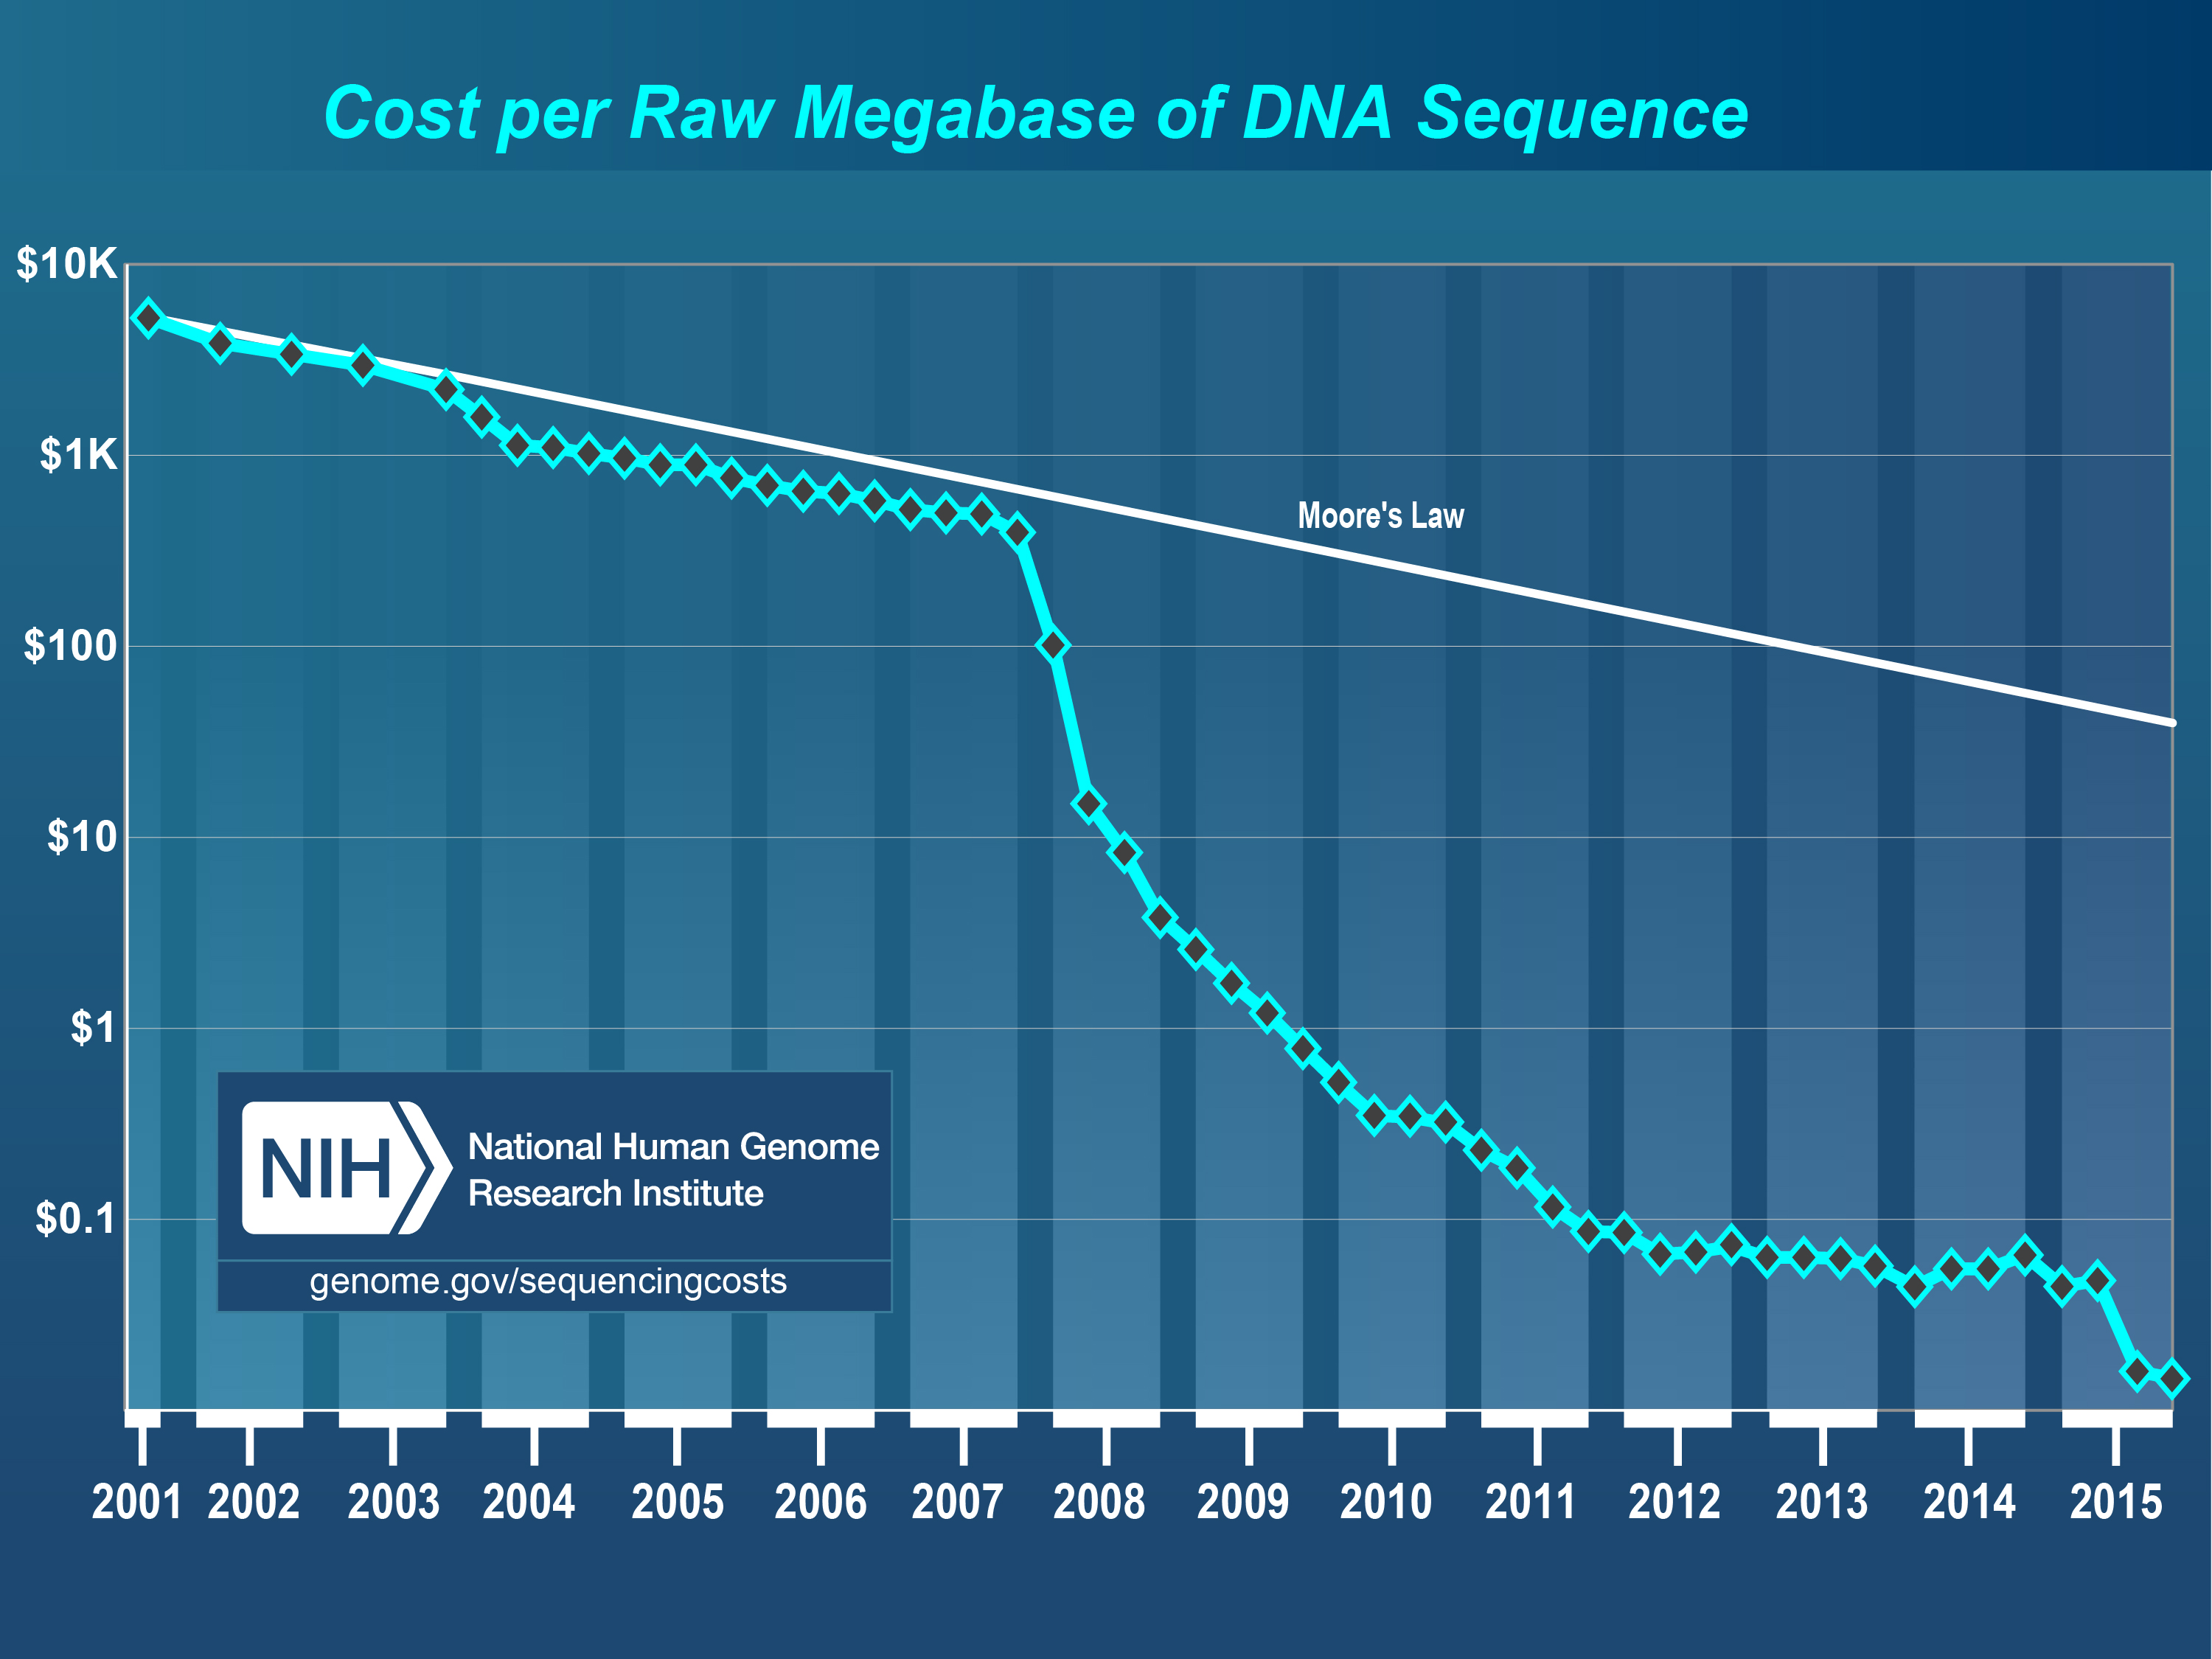
\includegraphics[scale=0.5]{costperMb2015_4.jpg}
\end{center}
\caption[Cost per raw megabase of DNA sequence from 2001 to 2015]{Cost per raw megabase of DNA sequence from 2001 to 2015. Straight line - Moore's Law, blue curve - cost in US dollars, Y-axis scale is logarithmic. Graph reproduced from \citep{wetterstrand2016}}
%Source:
\label{fig_dna_cost}
\end{figure}
Example of reference to a figure in the text (Fig.~\ref{fig_dna_cost}). Phasellus dolor neque, vehicula vestibulum semper at, facilisis eget libero. Mauris interdum magna molestie, auctor felis a, condimentum odio. Pellentesque habitant morbi tristique senectus et netus et malesuada fames ac turpis egestas. Suspendisse maximus lacinia dignissim. Maecenas pharetra accumsan metus, sagittis dictum purus sollicitudin eget. Curabitur ut porttitor arcu, ut porttitor ipsum. Vestibulum porttitor finibus sapien, ac pharetra odio bibendum nec. Nullam tincidunt dignissim risus imperdiet dictum.

Pellentesque habitant morbi tristique senectus et netus et malesuada fames ac turpis egestas. Suspendisse maximus lacinia dignissim. Maecenas pharetra accumsan metus, sagittis dictum purus sollicitudin eget. Curabitur ut porttitor arcu, ut porttitor ipsum. Vestibulum porttitor finibus sapien, ac pharetra odio bibendum nec. Nullam tincidunt dignissim risus imperdiet dictum.
\section{Example of a table}
Example of a table and here is the reference to Table \ref{table_genomes}. Tables in, my opinion, are the hardest thing to make.

\begin{table}
\begin{center}
\begin{tabular}{|l|c|c|c|}
\hline
{\sc Organism}  &  {\sc Accession no.}  & {\sc Genome size} (bp)  & {\sc No. CDS} \\
\hline
{\it Mesorhizobium loti}          & NC\_002678 & 7036071 & 6743 \\
\hline
{\it Sinorhizobium meliloti}      & NC\_003047 & 3654135 & 3359 \\
\hline
{\it Bradyrhizobium japonicum}    & NC\_004463 & 9105828 & 8317 \\
\hline
{\it Rhodopseudomonas palustris}  & NC\_005296 & 5459213 & 4813 \\
\hline
{\it Bartonella quintana}         & NC\_005955 & 1581384 & 1142 \\
\hline
{\it Bartonella henselae}         & NC\_005956 & 1931047 & 1488 \\
\hline
{\it Rickettsia typhi}            & NC\_006142 & 1111496 & 837 \\
\hline
{\it Beijerinckia indica}         & NC\_010581 & 4170153 & 3569 \\
\hline
\end{tabular}
\end{center}
\caption{Whole-genome sequences used in this study}
\label{table_genomes}
\end{table}

Fusce ultricies pulvinar diam sed ultrices. Sed orci justo, rutrum in dolor a, consequat dictum mi. Sed luctus congue ex nec dignissim. Phasellus volutpat urna vestibulum ipsum vestibulum, quis venenatis justo consectetur. Nullam hendrerit nisl in rutrum convallis. Sed sit amet malesuada nisi. Phasellus dolor neque, vehicula vestibulum semper at, facilisis eget libero. Mauris interdum magna molestie, auctor felis a, condimentum odio. Pellentesque habitant morbi tristique senectus et netus et malesuada fames ac turpis egestas. Suspendisse maximus lacinia dignissim. Maecenas pharetra accumsan metus, sagittis dictum purus sollicitudin eget. Curabitur ut porttitor arcu, ut porttitor ipsum. Vestibulum porttitor finibus sapien, ac pharetra odio bibendum nec. Nullam tincidunt dignissim risus imperdiet dictum.

Pellentesque habitant morbi tristique senectus et netus et malesuada fames ac turpis egestas. Suspendisse maximus lacinia dignissim. Maecenas pharetra accumsan metus, sagittis dictum purus sollicitudin eget. Curabitur ut porttitor arcu, ut porttitor ipsum. Vestibulum porttitor finibus sapien, ac pharetra odio bibendum nec. Nullam tincidunt dignissim risus imperdiet dictum.
\section{Chapter section}
Fusce ultricies pulvinar diam sed ultrices. Sed orci justo, rutrum in dolor a, consequat dictum mi. Sed luctus congue ex nec dignissim. Phasellus volutpat urna vestibulum ipsum vestibulum, quis venenatis justo consectetur. Nullam hendrerit nisl in rutrum convallis. Sed sit amet malesuada nisi. Phasellus dolor neque, vehicula vestibulum semper at, facilisis eget libero. Mauris interdum magna molestie, auctor felis a, condimentum odio. Pellentesque habitant morbi tristique senectus et netus et malesuada fames ac turpis egestas. Suspendisse maximus lacinia dignissim. Maecenas pharetra accumsan metus, sagittis dictum purus sollicitudin eget. Curabitur ut porttitor arcu, ut porttitor ipsum. Vestibulum porttitor finibus sapien, ac pharetra odio bibendum nec. Nullam tincidunt dignissim risus imperdiet dictum.

Pellentesque habitant morbi tristique senectus et netus et malesuada fames ac turpis egestas. Suspendisse maximus lacinia dignissim. Maecenas pharetra accumsan metus, sagittis dictum purus sollicitudin eget. Curabitur ut porttitor arcu, ut porttitor ipsum. Vestibulum porttitor finibus sapien, ac pharetra odio bibendum nec. Nullam tincidunt dignissim risus imperdiet dictum.

\include{}

% Bibliography
\begingroup
    \setlength\bibitemsep{10pt}
    \linespread{1}\selectfont
    \printbibliography[title=REFERENCES]
\endgroup
\addcontentsline{toc}{part}{REFERENCES}




% Appendices
\appendix

%%%%%%%%%% DON'T DELETE THIS, REVERTS NUMBERING BACK %%%%%%%%%%%%%
\makeatletter
\renewcommand{\@makechapterhead}[1]{\vspace *{-10\p@ }{\parindent \z@ 
\raggedright \normalfont \ifnum \c@secnumdepth >\m@ne \Huge \bfseries 
\@chapapp \space \thechapter \vskip 10\p@ \fi #1\par \nobreak \vskip 30\p@ }}
\makeatother
%%%%%%%%%% DON'T DELETE THIS, REVERTS NUMBERING BACK %%%%%%%%%%%%%


\include{content/appendix-1}

\end{document}
